\documentclass[11pt,a4paper]{article}
% Model documentation of leaf-conductance (build: see README.txt in this folder)
\usepackage[T1]{fontenc}
\usepackage[utf8]{inputenc}
\usepackage{lmodern}
% A4 with 2.5 cm margins (set directly; geometry.sty of the local TeX installation needs a newer kernel)
\setlength{\textwidth}{160mm}\setlength{\textheight}{237mm}
\setlength{\oddsidemargin}{-0.4mm}\setlength{\evensidemargin}{-0.4mm}
\setlength{\topmargin}{-0.4mm}\addtolength{\topmargin}{-\headheight}\addtolength{\topmargin}{-\headsep}
\setlength{\pdfpagewidth}{210mm}\setlength{\pdfpageheight}{297mm}
\usepackage{amsmath,amssymb}
\usepackage{graphicx}
\usepackage{booktabs,tabularx,longtable,multirow}
\usepackage{xcolor}
\usepackage[font=small,labelfont=bf]{caption}
\usepackage{enumitem}
\usepackage[round,authoryear]{natbib}
\usepackage[colorlinks=true,linkcolor=blue!50!black,citecolor=blue!50!black,urlcolor=blue!50!black]{hyperref}
\usepackage{listings}
\lstset{basicstyle=\ttfamily\small, columns=fullflexible, keepspaces=true, frame=single, rulecolor=\color{black!30}, backgroundcolor=\color{black!3}, xleftmargin=3pt, xrightmargin=3pt}
\providecommand{\doi}[1]{\href{https://doi.org/#1}{doi:\nolinkurl{#1}}}

\newcommand{\ExS}{25.133}
\newcommand{\ExDI}{1.091}
\newcommand{\ExLh}{12.966}
\newcommand{\ExLCo}{62.832}
\newcommand{\ExLi}{65.335}
\newcommand{\Exphi}{90.000}
\newcommand{\Extheta}{60.000}
\newcommand{\ExRa}{3.086\times10^{8}}
\newcommand{\ExNuc}{66.031}
\newcommand{\ExNuFU}{160.930}
\newcommand{\ExNuFL}{173.664}
\newcommand{\ExgbU}{3.457}
\newcommand{\ExgbL}{3.730}
\newcommand{\ExHU}{12.473}
\newcommand{\ExHL}{13.460}
\newcommand{\Exnu}{1.520}
\newcommand{\Exkappa}{2.148}
\newcommand{\Exrho}{1.198}
\newcommand{\ExLf}{32.300}
\newcommand{\Exphiw}{0.000}
\newcommand{\ExRef}{2125}
\newcommand{\ExgbmixU}{18.202}
\newcommand{\ExgbmixL}{18.213}
\newcommand{\Exfshare}{0.992}
\newcommand{\ExgbStillU}{3.480}
\newcommand{\ExgvStillU}{3.850}
\newcommand{\ExgcStillU}{2.695}
\newcommand{\ExkStillU}{0.845}
\newcommand{\ExgbStillL}{3.730}
\newcommand{\ExgvStillL}{4.127}
\newcommand{\ExgcStillL}{2.888}
\newcommand{\ExkStillL}{0.845}
\newcommand{\ExattStill}{9.115\times10^{-15}}
\newcommand{\ExwwStill}{U}
\newcommand{\ExgbWindU}{36.530}
\newcommand{\ExgvWindU}{39.560}
\newcommand{\ExgcWindU}{29.855}
\newcommand{\ExkWindU}{0.667}
\newcommand{\ExgbWindL}{36.532}
\newcommand{\ExgvWindL}{39.563}
\newcommand{\ExgcWindL}{29.857}
\newcommand{\ExkWindL}{0.667}
\newcommand{\ExattWind}{9.115\times10^{-15}}
\newcommand{\ExwwWind}{U}
\newcommand{\ExregimeWind}{laminar}
\newcommand{\ExRefWind}{6376}
\newcommand{\MaxDevEqNine}{0.03}
\newcommand{\LfOverLCo}{1.0281}
\newcommand{\LiOverLCo}{1.0395}
\newcommand{\LiFitOverLCo}{1.0398}
\newcommand{\ReLa}{\ensuremath{5\times10^{5}}}
\newcommand{\ReLb}{\ensuremath{3.63\times10^{5}}}
\newcommand{\ReLc}{\ensuremath{4.86\times10^{4}}}
\newcommand{\ReLd}{\ensuremath{2.04\times10^{4}}}
\newcommand{\ReLe}{\ensuremath{8.58\times10^{3}}}
\newcommand{\ReLf}{\ensuremath{2.73\times10^{3}}}
\newcommand{\GBmax}{1.196}
\newcommand{\GBmaxAt}{17.0}
\newcommand{\NRefCases}{121}
\newcommand{\NRefmixedCases}{320}
\newcommand{\NRefangleCases}{60}
\newcommand{\NRefscalarCases}{72}
\newcommand{\NRefTotal}{573}
\newcommand{\AngleRegimes}{40 laminar, 20 turbulent}
\newcommand{\PyDevFree}{1.5\times10^{-16}}
\newcommand{\PyDevMixed}{4.8\times10^{-16}}
\newcommand{\PyDevAngle}{5.3\times10^{-16}}
\newcommand{\PyDevScalar}{1.4\times10^{-17}}
\newcommand{\MlDevFree}{8.2\times10^{-16}}
\newcommand{\MlValsFree}{968}
\newcommand{\MlDevMixed}{4.8\times10^{-16}}
\newcommand{\MlValsMixed}{2880}
\newcommand{\MlDevAngle}{5.7\times10^{-16}}
\newcommand{\MlValsAngle}{480}
\newcommand{\MlDevScalar}{2.2\times10^{-16}}
\newcommand{\MlValsScalar}{864}
\newcommand{\MatlabVersion}{25.2.0.3042426 (R2025b) Update 1}
\newcommand{\PkgVersion}{1.1.0}
\newcommand{\NumpyVersion}{2.2.6}
\newcommand{\PythonVersion}{3.12.6}


\newcommand{\Nu}{\mathit{Nu}}
\newcommand{\NuF}{\mathit{Nu}_F}
\newcommand{\Ra}{\mathit{Ra}}
\newcommand{\Rey}{\mathit{Re}}
\newcommand{\Prn}{\mathit{Pr}}
\newcommand{\codeus}{\char95\allowbreak}
\DeclareRobustCommand{\code}[1]{\textnormal{\ttfamily\let\_\codeus #1}}
\emergencystretch=2em
\newcommand{\Gtt}[1]{G22~Eq.~#1}

\title{\textbf{leaf-conductance}\\[4pt]
\large Boundary-layer conductance of inclined elliptical leaves under free, forced and mixed convection\\[2pt]
\normalsize Model description, verification and validation\\[2pt]
\normalsize Software version \PkgVersion\ (Python and MATLAB)}
\author{Jan Graefe\\ \small Leibniz Institute of Vegetable and Ornamental Crops (IGZ), Gro\ss beeren, Germany}
\date{13 October 2026}

\begin{document}
\maketitle

\begin{abstract}
\noindent \texttt{leaf-conductance} computes the boundary-layer conductances of a flat elliptical leaf for heat, water vapour and CO$_2$, separately for the upper and the lower leaf side. Its core is the free-convection model of \citet{graefe2022}, which accounts for leaf size, aspect ratio and a two-axis inclination through flux-weighted characteristic lengths. The software extends this core by
(i)~a closed-form solution of the characteristic-length integral for elliptical leaves,
(ii)~laminar forced convection along the wind streamlines projected onto the leaf plane (flowline concept),
(iii)~the laminar--transitional--turbulent flat-plate correlation of \citet{lienhard2020} with a turbulence-dependent transition onset \citep{mayle1991},
(iv)~a five-parameter angle-of-attack model for the windward and leeward leaf side fitted to 815 literature measurements,
(v)~a turbulent branch of free convection,
(vi)~mixed convection by power-mean blending and
(vii)~mode-dependent conversion of the heat conductance to scalar conductances.
This document states every equation as implemented, the conventions of the two implementations, the test cases that verify them and the validation evidence, and it identifies the limits of validity. The Python and MATLAB implementations pass all 17 + 17 unit tests and agree on \NRefTotal\ shared reference cases to within $\ensuremath{1\times10^{-15}}$ relative deviation.
\end{abstract}

\tableofcontents
\newpage

%=====================================================================
\section{Introduction and scope}
%=====================================================================
The leaf boundary-layer conductance $g_b$ controls the exchange of sensible heat, water vapour and CO$_2$ between a leaf and the surrounding air and is therefore a central parameter of leaf energy-balance, transpiration and photosynthesis models. Simple formulations such as $g_b = |\Delta T|^{0.33}/400$ \citep{monteith1973} or the laminar flat-plate law $g_b \propto \sqrt{u/d}$ \citep{campbell1998} ignore the leaf shape and orientation and do not distinguish the two leaf sides. \citet{graefe2022} derived a free-convection model for inclined elliptical leaves from computational fluid dynamics, which resolves both effects.

The repository \texttt{leaf-conductance} provides this model in Python (single module \code{graefe\_convection.py}, NumPy only) and MATLAB (one function per file) and extends it to forced and mixed convection. Table~\ref{tab:origin} identifies which parts are taken from the peer-reviewed paper and which are extensions introduced in the software; the extensions have not been peer reviewed. Equation numbers of the paper are cited as ``\Gtt{x}''.

\begin{table}[ht]
\centering\small
\caption{Origin of the model components.}\label{tab:origin}
\begin{tabularx}{\textwidth}{>{\raggedright\arraybackslash}p{4.9cm}>{\raggedright\arraybackslash}X l}
\toprule
Component & Source & Section \\
\midrule
Geometry, characteristic lengths $L_h$, $L_i$ & \citet{graefe2022}, Eqs.~4--11, App.~A/B & \ref{sec:geometry} \\
Closed form of the flux-weighted length & extension (exact solution of \Gtt{4}) & \ref{sec:exactlength} \\
Laminar free convection, both sides & \citet{graefe2022}, Eqs.~1, 3a--3g, 14, 18, Table~3 & \ref{sec:free} \\
Turbulent free convection & extension & \ref{sec:freeturb} \\
Forced convection, flowline length & extension & \ref{sec:forced} \\
Laminar--turbulent transition & \citet{lienhard2020}, \citet{mayle1991}, \citet{kottke1977} & \ref{sec:lienhard} \\
Angle of attack, finite-plate factor & extension, fitted to literature data & \ref{sec:angle} \\
Mixed convection & extension (cubic power mean) & \ref{sec:mixed} \\
Heat, H$_2$O and CO$_2$ conductances & generalisation of \Gtt{17}; \citet{massman1998} & \ref{sec:scalar} \\
\bottomrule
\end{tabularx}
\end{table}

\paragraph{Notation and units.} All quantities are in SI units; temperatures in K, lengths in m, angles in degrees at the user interface. Table~\ref{tab:symbols} lists the symbols. The subscripts U and L denote the upper (adaxial in the horizontal position) and lower leaf side. Conductances and fluxes refer to one-sided leaf area.

\begin{table}[ht]
\centering\small
\caption{Principal symbols.}\label{tab:symbols}
\footnotesize
\begin{tabular}{lll@{\hspace{1.5em}}lll}
\toprule
Symbol & Meaning & Unit & Symbol & Meaning & Unit\\
\midrule
$L$, $W$ & leaf length, width ($L\ge W$) & m & $T_L$, $T_A$ & leaf, air temperature & K\\
$S$ & one-sided area & m$^2$ & $\Delta T$ & $T_L-T_A$ (or Eq.~\ref{eq:virtual}) & K\\
$AR$ & aspect ratio $L/W$ & -- & $u$ & wind speed & m\,s$^{-1}$\\
$\alpha_x$, $\alpha_y$ & rotations about short / long axis & deg & TI & turbulence intensity & \%\\
$\theta$ & angle leaf normal -- vertical & rad & $\nu$ & kinematic viscosity & m$^2$\,s$^{-1}$\\
$\varphi$ & streamline angle to short axis & rad & $\kappa$ & thermal diffusivity & m$^2$\,s$^{-1}$\\
$L_h$, $L_i$ & char.\ lengths, horizontal / inclined & m & $\rho$, $c_p$ & air density, heat capacity & --\\
$L_{Co}$ & mean chord length & m & $\NuF$ & flux-proportional Nusselt no. & m$^{-1}$\\
$L_f$ & forced-convection streamline length & m & $\Ra$ & Rayleigh number per m$^3$ & m$^{-3}$\\
$\beta$ & angle of attack & deg & $g_b$, $g_v$, $g_c$ & conductance heat, H$_2$O, CO$_2$ & m\,s$^{-1}$\\
\bottomrule
\end{tabular}
\end{table}

%=====================================================================
\section{Physical basis}\label{sec:basis}
%=====================================================================
\subsection{Conductance and flux-proportional Nusselt number}
Following \citet{graefe2022}, the Nusselt number is expressed without a length scale, $\NuF = h/k$ (m$^{-1}$), where $h$ is the heat-transfer coefficient and $k$ the thermal conductivity of air. The conductance for heat and the sensible heat flux of one leaf side are then (\Gtt{1}, \Gtt{14})
\begin{equation}
g_b = \kappa\,\NuF, \qquad H = \rho\,c_p\,g_b\,(T_L - T_A),\label{eq:gb}
\end{equation}
with $H>0$ from leaf to air. A conventional dimensionless Nusselt number based on a length $\ell$ is $\Nu_\ell = \NuF\,\ell$. This formulation allows terms with different characteristic lengths to be combined.

\subsection{Air properties}
All air properties are evaluated at the film temperature $T_F = (T_L+T_A)/2$ for dry air (\code{air\_properties}, \code{airProperties.m}):
\begin{align}
\rho &= \frac{p}{R_d T_F}, \quad R_d = 287.05\,J\,kg\ensuremath{^{-1}}\,K\ensuremath{^{-1}},\\
\mu &= \frac{\ensuremath{1.458\times10^{-6}}\,T_F^{1.5}}{T_F + 110.4}\ \text{(Sutherland's law; \citealp{sutherland1893})},\qquad \nu = \mu/\rho,\\
k &= 0.02624\,(T_F/300)^{0.8646}, \qquad \kappa = k/(\rho\,c_p),\quad c_p = 1004\,J\,kg\ensuremath{^{-1}}\,K\ensuremath{^{-1}},
\end{align}
with $\Prn = 0.71$ and $g = 9.81\,m\,s\ensuremath{^{-2}}$ held constant. At 20\,\ensuremath{^\circ}C and 101325\,Pa these give $\rho = 1.204$\,kg\,m$^{-3}$, $\nu = \ensuremath{1.51\times10^{-5}}$ and $\kappa = \ensuremath{2.12\times10^{-5}}$\,m$^2$\,s$^{-1}$ (test \code{test\_air\_properties\_20C}).

%=====================================================================
\section{Leaf geometry and characteristic lengths}\label{sec:geometry}
%=====================================================================
\subsection{Ellipse, dissection index and horizontal leaf}
The leaf is a flat ellipse with axes $L\ge W$ (\code{leaf\_geometry}, \code{leafGeometry.m}); $L<W$ raises an error. Its area is $S = \tfrac{\pi}{4}LW$ and its aspect ratio $AR = L/W$. The perimeter is expressed through the dissection index (\Gtt{8}, maximum error 0.04\,\% for $AR = 1$--4)
\begin{equation}
DI = 1.112\left(\frac{L+W}{\sqrt{LW}}\right)^{0.783} - 0.913, \qquad P = 2\,DI\sqrt{\pi S},
\end{equation}
and the characteristic length of the horizontal leaf is (\Gtt{7})
\begin{equation}
L_h = \frac{S}{P} = \frac{\sqrt{S}}{2\,DI\sqrt{\pi}} .
\end{equation}
For a circle $DI=1$ and $L_h = D/4$.

\subsection{Inclination and streamline direction}
The unrotated leaf has its short axis along $x$, its long axis along $y$ and its normal along $z$ (up). It is first rotated about $y$ by $\alpha_y$ and then about $x$ by $\alpha_x$, $\mathbf{R} = \mathbf{R}_x(\alpha_x)\,\mathbf{R}_y(\alpha_y)$ (App.~B of \citealp{graefe2022}). The rotated normal $\mathbf{n} = \mathbf{R}\hat{\mathbf z}$ subtends the angle
\begin{equation}
\cos\theta = \cos\alpha_x\cos\alpha_y \qquad\text{(\Gtt{11})}
\end{equation}
with the vertical. Buoyancy-driven streamlines follow the steepest-ascent direction $\mathbf s = \hat{\mathbf z} - (\hat{\mathbf z}\cdot\mathbf n)\mathbf n$ in the leaf plane; its angle to the rotated short axis $\mathbf w = \mathbf R\hat{\mathbf x}$ is
\begin{equation}
\varphi = \arccos\frac{|\mathbf s\cdot\mathbf w|}{\lVert\mathbf s\rVert}\in[0,\pi/2].
\end{equation}
For $\alpha_y = 0$ the flow runs along the long axis ($\varphi = \pi/2$). For a horizontal leaf $\mathbf s = \mathbf 0$ and $\varphi = \pi/2$ is returned by convention (the inclined term vanishes with $\sin\theta = 0$).

\subsection{Mean chord length and characteristic length of the inclined leaf}
The mean length of the chords parallel to the streamline direction is (\Gtt{9}, App.~A; written with $\sin/\cos$ to remain finite at $\varphi=\pi/2$)
\begin{equation}
L_{Co}(\varphi) = \frac{\pi L W}{4\sqrt{(W\sin\varphi)^2 + (L\cos\varphi)^2}},
\end{equation}
and the characteristic length of the inclined leaf is the linear fit (\Gtt{9})
\begin{equation}
L_i = (0.04511\,n + 1.006)\,L_{Co}(\varphi), \qquad n = 3\times 0.25 = 0.75 .\label{eq:Li}
\end{equation}
For $\alpha_y=0$, $L_i = 0.816\,L$. Figure~\ref{fig:charlength}a shows $L_{Co}$ over $\varphi$.

\begin{figure}[ht]
\centering
\begin{minipage}{0.46\textwidth}\centering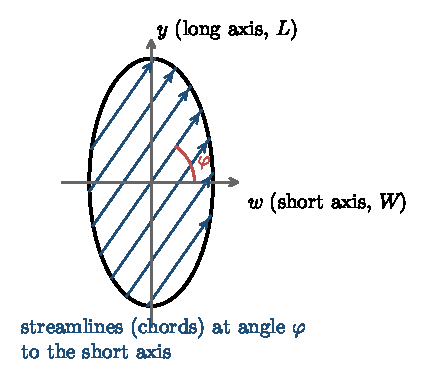
\includegraphics[width=\linewidth]{fig/geometry.pdf}\end{minipage}\hfill
\begin{minipage}{0.5\textwidth}
\caption{Leaf in its own plane. Streamlines (chords) at the angle $\varphi$ to the short axis; along the chord at offset $t$ the boundary layer develops over the length $D(t)$. Free convection uses the steepest-ascent direction, forced convection the wind direction projected onto the leaf plane.}\label{fig:geometry}
\end{minipage}
\end{figure}

\subsection{Closed form of the flux-weighted characteristic length}\label{sec:exactlength}
\Gtt{4} defines the characteristic length as the length for which a uniform transfer law $h\propto \ell^{\,n-1}$ (local Nusselt number $\propto \ell^{\,n}$) yields the same total flux as the integral over all chords. For an ellipse the chords parallel to any direction have the lengths $D(t) = D_0\sqrt{1-(t/t_{\max})^2}$, with $D_0 = \tfrac{4}{\pi}L_{Co}(\varphi)$ the longest chord. Substituting $t = t_{\max}\sin\psi$ gives
\begin{equation}
\frac{\int D(t)^{n}\,\mathrm dt}{\int D(t)\,\mathrm dt} = D_0^{\,n-1}\,\frac{\int_0^{\pi/2}\cos^{n+1}\psi\,\mathrm d\psi}{\int_0^{\pi/2}\cos^{2}\psi\,\mathrm d\psi}
\;\Rightarrow\;
L_c^{\,n-1} = D_0^{\,n-1}\,\frac{2}{\pi}\,B\!\left(\tfrac12,\tfrac n2+1\right),\label{eq:exact}
\end{equation}
with the Beta function $B$ (\code{characteristic\_length}, \code{characteristicLength.m}; for $n=1$ the mean chord length is returned). Because the chord distribution of an ellipse is self-similar, $L_c/L_{Co}$ depends only on $n$ and not on $\varphi$ or $AR$:
\begin{itemize}[nosep]
\item $n = 0.75$ (laminar free convection, $\Nu\propto\Ra^{1/4}$): $L_c/L_{Co} = \LiOverLCo$; the fit of Eq.~\eqref{eq:Li} gives \LiFitOverLCo, i.e.\ the paper's regression is reproduced within \MaxDevEqNine\,\% for all $\varphi$ and $AR$ (Fig.~\ref{fig:charlength}b).
\item $n = 0.5$ (laminar forced convection, $h\propto\ell^{-1/2}$): $L_f/L_{Co} = \LfOverLCo$.
\end{itemize}
The model keeps the published fit (Eq.~\ref{eq:Li}) for free convection and uses Eq.~\eqref{eq:exact} with $n=0.5$ for forced convection.

\begin{figure}[ht]
\centering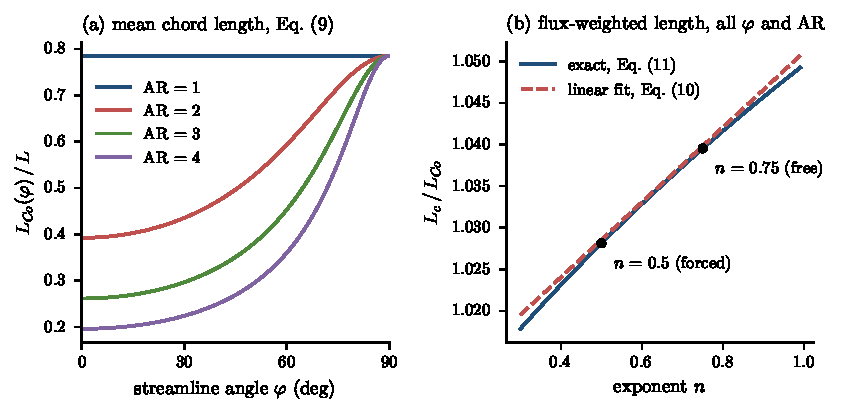
\includegraphics[width=\textwidth]{fig/charlength.pdf}
\caption{(a) Mean chord length $L_{Co}$ relative to the leaf length for aspect ratios 1--4. (b) Ratio of the flux-weighted characteristic length to the mean chord length over the exponent $n$: closed form Eq.~\eqref{eq:exact} and the linear fit Eq.~\eqref{eq:Li}. The ratio is the same for all streamline angles and aspect ratios; at $n = 0.75$ fit and closed form differ by \MaxDevEqNine\,\%.}\label{fig:charlength}
\end{figure}

%=====================================================================
\section{Free convection}\label{sec:free}
%=====================================================================
\subsection{Laminar model of Graefe et al. (2022)}
With the Rayleigh number per unit volume (\Gtt{3g}; buoyancy coefficient $1/T_A$, $\nu$ at film temperature)
\begin{equation}
\Ra = \frac{g\,|\Delta T|\,\Prn}{T_A\,\nu^2}\quad[\mathrm m^{-3}],
\end{equation}
the contributions of the inclined (i) and horizontal (h) components for a \emph{heated} leaf ($\Delta T>0$) are (\Gtt{3b}--\Gtt{3e})
\begin{align}
\Nu_{i,U} &= p_3\,L_i^{-1/4}\,\sin^{p_4}\theta\;\Ra^{1/4}, &
\Nu_{i,L} &= p_3\,L_i^{-1/4}\,\sin^{1/4}\theta\;\Ra^{1/4},\\
\Nu_{h,U} &= p_5\,L_h^{-1/4}\,\cos^{1/4}\theta\;\Ra^{1/4}, &
\Nu_{h,L} &= p_6\,L_h^{-0.4}\,\cos^{0.2}\theta\;\Ra^{0.2},
\end{align}
the conduction limit of the elliptical plate (\Gtt{3f}; \citealp{yovanovich1998}) is
\begin{equation}
\Nu_c = \frac{5.3\,\sin(0.0338\,AR + 0.607)}{\sqrt S},
\end{equation}
and the side-specific flux-proportional Nusselt number is the nested power mean (\Gtt{3a})
\begin{equation}
\NuF = \Big\{\big[\Nu_i^{\,p_1} + \Nu_h^{\,p_1}\big]^{p_2/p_1} + \Nu_c^{\,p_2}\Big\}^{1/p_2}.\label{eq:free}
\end{equation}
For a \emph{cooled} leaf ($\Delta T<0$) the right-hand sides of U and L are exchanged, since the lower side then faces the unstable stratification. The parameters (Table~3 of the paper) are $p_1 = 6$, $p_2 = 1.42$, $p_3 = 0.513$, $p_4 = 0.4$, $p_5 = 0.202$, $p_6 = 0.492$. Implementation: \code{free\_convection}, \code{nusselt\_free} / \code{graefeFreeConvection.m}. To avoid a singularity at $\Delta T=0$, $|\Delta T|$ is bounded below by \ensuremath{10^{-9}}\,K.

\paragraph{Vapour buoyancy.} If leaf-surface and air vapour pressures $e_L$, $e_A$ are supplied, the buoyancy uses the virtual temperature difference (\Gtt{18})
\begin{equation}
\Delta T' = \Delta T + 0.38\,\frac{e_L T_L - e_A T_A}{p},\label{eq:virtual}
\end{equation}
so that a transpiring leaf slightly cooler than the air may still drive upward convection. The heat flux in Eq.~\eqref{eq:gb} always uses the actual $T_L-T_A$.

\begin{figure}[ht]
\centering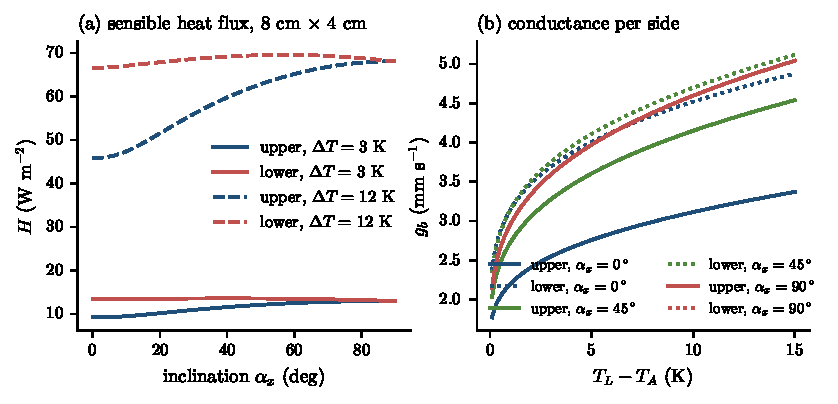
\includegraphics[width=\textwidth]{fig/free.pdf}
\caption{Laminar free convection of an $8\times4$\,cm leaf at $T_A = 20\,\ensuremath{^\circ}C$. (a) Sensible heat flux of both sides over the inclination $\alpha_x$ ($\alpha_y = 0$), cf.\ Fig.~6b of \citet{graefe2022}: the sides converge with increasing inclination and are identical for the vertical leaf. (b) Conductance per side over the temperature difference.}\label{fig:free}
\end{figure}

\subsection{Extension: turbulent free convection}\label{sec:freeturb}
For large or hot leaves the buoyant boundary layer on the unstable side becomes turbulent, where the heat transfer becomes independent of the length scale. \code{free\_convection\_transition} / \code{freeConvectionTransition.m} add
\begin{equation}
\mathit{Nu}_{F,\mathrm{turb}} = 0.14\,\Ra^{1/3},\qquad
\NuF = \big(\mathit{Nu}_{F,\mathrm{lam}}^{\,6} + \mathit{Nu}_{F,\mathrm{turb}}^{\,6}\big)^{1/6}
\end{equation}
on the buoyantly unstable side (upper side of a heated, lower side of a cooled leaf, both sides of a vertical leaf). The stably stratified side keeps its laminar value. The turbulent share $s_t = \mathit{Nu}_{F,\mathrm{turb}}^6/(\mathit{Nu}_{F,\mathrm{lam}}^6+\mathit{Nu}_{F,\mathrm{turb}}^6)$ is reported for the scalar exponent (Section~\ref{sec:scalar}). For leaf-sized objects $s_t$ is negligible (e.g.\ $<2\,\%$ change for an $8\times4$\,cm leaf at $\Delta T = 1$\,K); the branch matters for leaves of decimetre size and $\Delta T\gtrsim 10$\,K.

%=====================================================================
\section{Forced convection}\label{sec:forced}
%=====================================================================
\subsection{Wind geometry and flowline length}
The horizontal wind blowing from the meteorological direction $\delta$ (\code{wind\_from\_deg}) has the direction vector $\mathbf d$ towards azimuth $\delta+180^\circ$. The leaf azimuth $A$ (\code{leaf\_azimuth\_deg}) is the compass direction that the upper surface faces (180 = south); before tilting, the long axis points horizontally towards $A+180^\circ$ (up-slope) and the short axis is perpendicular to it. Expressed in the leaf frame, $\mathbf d$ is projected onto the leaf plane,
\begin{equation}
\mathbf d_p = \mathbf d - (\mathbf d\cdot\mathbf n)\,\mathbf n,\qquad
\varphi_w = \arccos\frac{|\mathbf d_p\cdot\mathbf w|}{\lVert\mathbf d_p\rVert},\qquad
\beta = \arcsin|\mathbf d\cdot\mathbf n|,
\end{equation}
where $\varphi_w$ is the streamline angle to the short axis (\code{wind\_streamline\_angle}), $\lVert\mathbf d_p\rVert$ the in-plane fraction of the wind and $\beta$ the angle of attack (\code{wind\_attack\_angle}); the windward side is U if $\mathbf d\cdot\mathbf n<0$, otherwise L. The streamline length for laminar forced convection is Eq.~\eqref{eq:exact} with $n = 0.5$,
\begin{equation}
L_f = L_c(\varphi_w;\,n = 0.5)\qquad(\code{forced\_length}).
\end{equation}
If the wind direction is unknown (\code{wind\_from\_deg=None} / \code{[]}) or the wind is normal to the leaf ($\lVert\mathbf d_p\rVert<10^{-6}$), the orientation-averaged chord length $\pi S/P$ (\Gtt{5}) replaces $L_{Co}$, i.e.\ $D_0 = 4S/P$. The full wind speed $u$ is used in the Reynolds number; the in-plane fraction is reported but not applied.

\subsection{Laminar flat plate}
In the basic forced model (\code{nusselt\_forced} with \code{transition=False}) each side follows the laminar flat-plate law \citep{pohlhausen1921}
\begin{equation}
\mathit{Nu}_{F,\mathrm{forced}} = \frac{c\,\Rey^{1/2}\,\Prn^{1/3}}{L_f},\qquad \Rey = \frac{u L_f}{\nu},\qquad c = 0.664 .
\end{equation}
(\citet{campbell1998} use $c=0.6$; the coefficient can be passed as \code{c\_forced}.)

\subsection{Laminar--turbulent transition}\label{sec:lienhard}
\code{forced\_nusselt\_lienhard} / \code{forcedNusseltLienhard.m} implement the average Nusselt number of \citet{lienhard2020}. The local laws are
\begin{align}
\text{laminar } (\Rey_x\le\Rey_l):&\quad \Nu_x = a_l\,\Rey_x^{1/2}\Prn^{1/3},\quad a_l = 0.332,\\
\text{transitional } (\Rey_l<\Rey_x\le\Rey_u):&\quad \Nu_x = \Nu_x(\Rey_l)\,(\Rey_x/\Rey_l)^{c},\quad c = 0.9922\log_{10}\Rey_l - 3.013,\\
\text{turbulent } (\Rey_x>\Rey_u):&\quad \Nu_x = 0.0296\,\Rey_x^{0.8}\Prn^{0.6}.
\end{align}
The end of transition $\Rey_u$ follows from continuity of $\Nu_x$ at $\Rey_u$,
\begin{equation}
\Rey_u = \left[\frac{a_l}{0.0296}\,\Rey_l^{\,1/2-c}\,\Prn^{1/3-0.6}\right]^{1/(0.8-c)},
\end{equation}
and the plate average $\overline{\Nu} = \int_0^{\Rey}\Nu_x\,\Rey_x^{-1}\,\mathrm d\Rey_x$ is evaluated exactly:
\begin{equation}
\begin{split}
\overline{\Nu} = {}& 2a_l\Prn^{1/3}\min(\Rey,\Rey_l)^{1/2}
+ \frac{\Nu_x(\Rey_l)}{c}\left[\left(\frac{\min(\Rey,\Rey_u)}{\Rey_l}\right)^{c}-1\right]_{\Rey>\Rey_l}\\
&+ 0.037\,\Prn^{0.6}\left[\Rey^{0.8}-\Rey_u^{0.8}\right]_{\Rey>\Rey_u}.
\end{split}\label{eq:lienhard}
\end{equation}
For a uniform-heat-flux plate the laminar average coefficient becomes 0.680 instead of 0.664 (\code{bc="uniform\_flux"}); an unheated starting length $x_0$ multiplies the laminar part by $[1-(x_0/L)^{3/4}]^{-1/3}$.

\paragraph{Transition onset.} The onset depends on the free-stream turbulence intensity. Mayle's (\citeyear{mayle1991}) correlation $\Rey_{\theta,t} = 400\,\mathrm{TI}^{-5/8}$, converted with the Blasius momentum thickness $\Rey_\theta = 0.664\,\Rey_x^{1/2}$, gives
\begin{equation}
\Rey_l = 3.63\times10^{5}\,\mathrm{TI}^{-1.25},\qquad \ensuremath{2\times10^{3}}\le\Rey_l\le\ensuremath{5\times10^{5}}\qquad(\code{transition\_onset\_reynolds}).
\end{equation}
Example values: TI = 0.1\,\% $\to$ \ReLa (cap), 1\,\% $\to$ \ReLb, 5\,\% $\to$ \ReLc, 10\,\% $\to$ \ReLd, 20\,\% $\to$ \ReLe, 50\,\% $\to$ \ReLf. In canopies (TI 20--50\,\%) leaves of a few centimetres can therefore reach transitional flow at moderate wind speeds. The regime is reported as \code{forced\_regime} (laminar / transitional / turbulent).

\paragraph{Blunt leading edges.} If $\Rey_t = u\,t/\nu\ge 2000$ for a plate of thickness $t$ \citep{kottke1977}, the boundary layer is tripped at the edge and \code{forced\_nusselt\_turbulent} gives $\overline{\Nu} = 0.037\,\Rey^{0.8}\Prn^{0.6}$. Thin leaves do not reach this criterion; it is provided for thick test bodies only and is not used in the general model.

\begin{figure}[ht]
\centering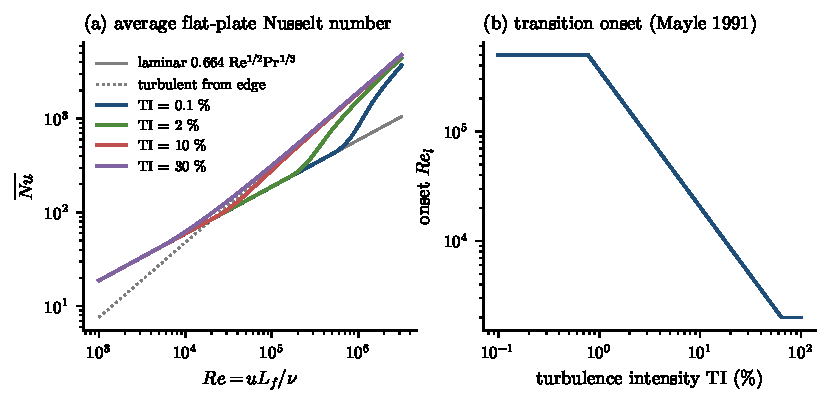
\includegraphics[width=\textwidth]{fig/lienhard.pdf}
\caption{(a) Average flat-plate Nusselt number (Eq.~\ref{eq:lienhard}) for several turbulence intensities, with the laminar and fully turbulent limits. (b) Transition onset Reynolds number after \citet{mayle1991}, bounded to $[\ensuremath{2\times10^{3}},\ensuremath{5\times10^{5}}]$.}\label{fig:lienhard}
\end{figure}

\subsection{Extension: angle of attack and finite-plate enhancement}\label{sec:angle}
Inclined to the wind, the windward side of a thin plate experiences an accelerated outer flow, while the leeward side is first covered by a reattaching separation bubble (enhancement at small angles) and at larger angles by a wake (reduction). A parsimonious model with five parameters describes both sides (\code{angle\_of\_attack\_factors}, \code{forced\_nusselt\_leaf} / \code{angleOfAttackFactors.m}, \code{forcedNusseltLeaf.m}):
\begin{align}
\overline{\Nu}_0 &= f_e\,\overline{\Nu}_{\mathrm{plate}}(\Rey,\mathrm{TI}),\\
\text{windward:}\quad \overline{\Nu}_W &= \overline{\Nu}_0\,g_W,\qquad g_W = 1 + a_W\sin\beta,\\
\text{leeward:}\quad \overline{\Nu}_B &= \overline{\Nu}_0\,g_B,\qquad g_B = w\,(1 + a_R\sin2\beta) + (1-w)\,c_w,\\
 w &= \exp\!\big[-(\beta/\beta_s)^2\big],
\end{align}
where $\overline{\Nu}_{\mathrm{plate}}$ is Eq.~\eqref{eq:lienhard} and $f_e$ accounts for edge effects and three-dimensional flow on finite plates. The fitted values are given in Table~\ref{tab:angleparams}. In parallel flow both factors are 1; the leeward factor peaks at $g_B = \GBmax$ at $\beta = \GBmaxAt^\circ$ and tends to $c_w<1$ in normal flow (Fig.~\ref{fig:angle}).

\begin{figure}[ht]
\centering
\begin{minipage}{0.48\textwidth}\centering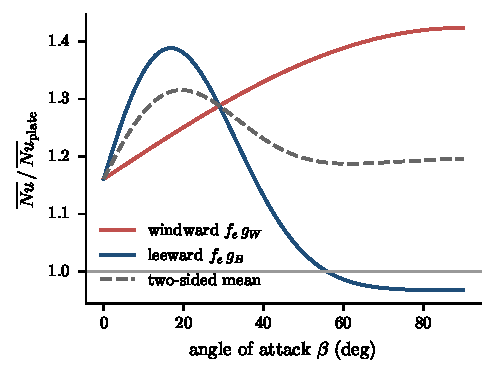
\includegraphics[width=\linewidth]{fig/angle.pdf}\end{minipage}\hfill
\begin{minipage}{0.48\textwidth}
\caption{Angle-of-attack model: average Nusselt number of the windward and leeward side relative to the infinite flat plate in parallel flow, including the finite-plate factor $f_e = 1.161$.}\label{fig:angle}
\end{minipage}
\end{figure}

%=====================================================================
\section{Mixed convection}\label{sec:mixed}
%=====================================================================
Free and forced contributions are combined per side by the cubic power mean
\begin{equation}
\mathit{Nu}_{F,\mathrm{mix}} = \big(\mathit{Nu}_{F,\mathrm{free}}^{\,3} + \mathit{Nu}_{F,\mathrm{forced}}^{\,3}\big)^{1/3},\qquad
s_f = \frac{\mathit{Nu}_{F,\mathrm{forced}}^{\,3}}{\mathit{Nu}_{F,\mathrm{free}}^{\,3}+\mathit{Nu}_{F,\mathrm{forced}}^{\,3}},
\end{equation}
where $s_f$ is the forced share (\code{mixed\_convection} / \code{graefeMixedConvection.m}). Assisting and opposing flows are not distinguished. Options select the transition model (\code{transition}, \code{TI\_pct}), the angle-of-attack model (\code{angle\_model}; the windward side receives $g_W$, the other side $g_B$) and the turbulent free-convection branch (\code{free\_transition}). Without wind ($u=0$) the result is identical to pure free convection.

%=====================================================================
\section{Conductances for heat, water vapour and CO\texorpdfstring{$_2$}{2}}\label{sec:scalar}
%=====================================================================
For a transfer law $\Nu\propto \Prn^{m}$ (or $Sc^{m}$), the conductance for a scalar with molecular diffusivity $D_s$ is
\begin{equation}
g_s = g_b\,(D_s/\kappa)^{k},\qquad k = 1 - m .
\end{equation}
The exponent differs between transport modes (Table~\ref{tab:kexp}). The general model (\code{leaf\_conductances} / \code{leafConductances.m}) uses the share-weighted mean, generalising \Gtt{17}:
\begin{align}
s_c &= \Nu_c/\max(\mathit{Nu}_{F,\mathrm{lam}},\Nu_c), & k_{\mathrm{free,lam}} &= 0.75 + 0.25\,s_c,\\
k_{\mathrm{free}} &= (1-s_t)\,k_{\mathrm{free,lam}} + s_t\cdot\tfrac23, &
k_{\mathrm{forced}} &= (1-f_t)\cdot\tfrac23 + f_t\cdot0.4,\\
k &= (1-s_f)\,k_{\mathrm{free}} + s_f\,k_{\mathrm{forced}},
\end{align}
with the conduction share $s_c$, the turbulent free share $s_t$ (Section~\ref{sec:freeturb}), the turbulent forced share $f_t$ = turbulent part / total of Eq.~\eqref{eq:lienhard}, and the forced share $s_f$. The diffusivities \citep{massman1998} are
\begin{equation}
D_{\mathrm{H_2O}} = \ensuremath{2.12\times10^{-5}}\,f,\qquad D_{\mathrm{CO_2}} = \ensuremath{1.39\times10^{-5}}\,f\quad[\mathrm m^2\,\mathrm s^{-1}],\qquad
f = \left(\frac{T_F}{273.15}\right)^{1.75}\frac{101325}{p}.
\end{equation}
Since $D_{\mathrm{H_2O}}>\kappa>D_{\mathrm{CO_2}}$, $g_v>g_b>g_c$ always.

\begin{table}[ht]
\centering\small
\caption{Diffusivity exponent $k$ of the transport modes.}\label{tab:kexp}
\begin{tabular}{llc}
\toprule
Mode & Law & $k$\\
\midrule
Conduction limit & $\Nu = \mathrm{const}$ & 1\\
Laminar free convection & $\Nu\propto\Ra^{1/4}$ & 3/4\\
Turbulent free convection & $\Nu\propto\Ra^{1/3}$ & 2/3\\
Forced, laminar and transitional & $\Nu\propto\Prn^{1/3}$ & 2/3\\
Forced, turbulent & $\Nu\propto\Prn^{0.6}$ & 0.4\\
\bottomrule
\end{tabular}
\end{table}

\begin{figure}[ht]
\centering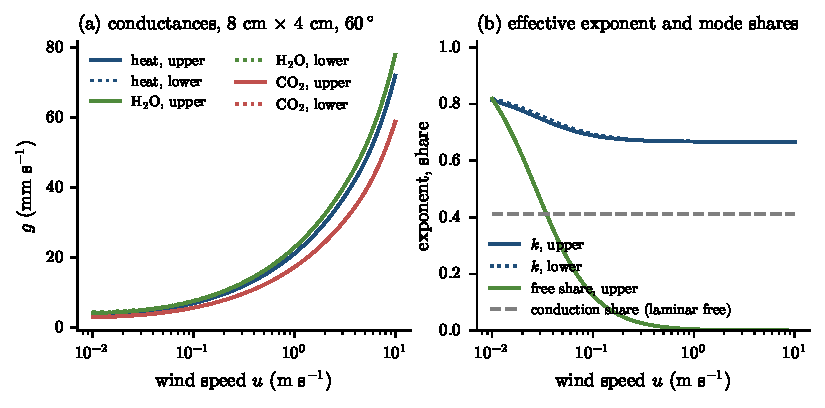
\includegraphics[width=\textwidth]{fig/general.pdf}
\caption{General model for an $8\times4$\,cm leaf inclined by $60^\circ$, $\Delta T = 3$\,K, $T_A = 20\,\ensuremath{^\circ}C$, wind from the west (along the short axis, $\beta = 0$), TI = 20\,\%. (a) Conductances for heat, H$_2$O and CO$_2$ of both sides over the wind speed. (b) Effective exponent $k$, free share and conduction share.}\label{fig:general}
\end{figure}

%=====================================================================
\section{Implementation}\label{sec:impl}
%=====================================================================
\subsection{Structure and interfaces}
Both implementations share the same formulation and parameter values; Table~\ref{tab:api} maps the functions. Temperatures, vapour pressures and wind speed may be arrays (elementwise evaluation); the geometry is scalar. All functions return dictionaries (Python) or structs (MATLAB) containing the side-specific results and the intermediate quantities.

\begin{table}[ht]
\centering\small
\caption{Functions of the Python module \code{graefe\_convection} and the MATLAB folder.}\label{tab:api}
\begin{tabularx}{\textwidth}{l l >{\raggedright\arraybackslash}X}
\toprule
Python & MATLAB & Purpose\\
\midrule
\code{air\_properties} & \code{airProperties} & $\rho$, $\nu$, $\kappa$, $k$\\
\code{leaf\_geometry} & \code{leafGeometry} & $S$, $AR$, $DI$, $P$, $L_h$, $\theta$, $\varphi$, $L_{Co}$, $L_i$\\
\code{characteristic\_length} & \code{characteristicLength} & closed form Eq.~\eqref{eq:exact}\\
\code{wind\_streamline\_angle} & \code{windStreamlineAngle} & $\varphi_w$, in-plane fraction\\
\code{wind\_attack\_angle} & \code{windAttackAngle} & $\beta$, windward side\\
\code{free\_convection} & \code{graefeFreeConvection} & laminar free convection (paper)\\
\code{free\_convection\_transition} & \code{freeConvectionTransition} & with turbulent branch\\
\code{forced\_nusselt\_lienhard} & \code{forcedNusseltLienhard} & Eq.~\eqref{eq:lienhard}\\
\code{angle\_of\_attack\_factors} & \code{angleOfAttackFactors} & $g_W$, $g_B$\\
\code{forced\_nusselt\_leaf} & \code{forcedNusseltLeaf} & windward/leeward Nusselt numbers\\
\code{mixed\_convection} & \code{graefeMixedConvection} & free + forced, per side\\
\code{leaf\_conductances} & \code{leafConductances} & general model, heat/H$_2$O/CO$_2$\\
\bottomrule
\end{tabularx}
\end{table}

\paragraph{Defaults.} \code{mixed\_convection} defaults to the laminar forced law without angle model. \code{leaf\_conductances} enables all extensions (\code{transition}, \code{free\_transition}, \code{angle\_model} = true) with TI = 1\,\% unless specified.

\paragraph{Usage.} Python and MATLAB calls of the general model:
\begin{lstlisting}[language=Python]
from graefe_convection import leaf_conductances
r = leaf_conductances(TL=296.15, TA=293.15, u=1.5, L=0.08, W=0.04,
                      alpha_x_deg=60, leaf_azimuth_deg=180,
                      wind_from_deg=270, TI_pct=20)
r["gb_U"], r["gv_U"], r["gc_U"], r["k_U"]   # m/s, upper side
\end{lstlisting}
\begin{lstlisting}
r = leafConductances(296.15, 293.15, 1.5, 0.08, 0.04, 60, 0, 180, 270, ...
                     [], [], [], 20);
\end{lstlisting}

\subsection{Worked example}
Table~\ref{tab:example} documents intermediate and final values for an $8\times4$\,cm leaf inclined by $\alpha_x = 60^\circ$, $T_L = 23\,\ensuremath{^\circ}C$, $T_A = 20\,\ensuremath{^\circ}C$, $p = 101325\,Pa$, facing south, so that users can check other implementations.

\begin{table}[ht]
\centering\small
\caption{Worked example (8\,cm $\times$ 4\,cm, $\alpha_x = 60^\circ$, $\alpha_y = 0$, $\Delta T = 3$\,K, $T_A = 293.15$\,K).}\label{tab:example}
\footnotesize
\begin{tabular}{lr@{\hspace{2.5em}}lr}
\toprule
\multicolumn{2}{l}{Geometry and air} & \multicolumn{2}{l}{Free convection (laminar, paper)}\\
\midrule
$S$ (cm$^2$) & \ExS & $\Ra$ (m$^{-3}$) & $\ExRa$\\
$DI$ & \ExDI & $\Nu_c$ (m$^{-1}$) & \ExNuc\\
$L_h$ (mm) & \ExLh & $\mathit{Nu}_{F,U}$ / $\mathit{Nu}_{F,L}$ (m$^{-1}$) & \ExNuFU\ / \ExNuFL\\
$L_{Co}$ / $L_i$ (mm) & \ExLCo\ / \ExLi & $g_{b,U}$ / $g_{b,L}$ (mm\,s$^{-1}$) & \ExgbU\ / \ExgbL\\
$\theta$ / $\varphi$ (deg) & \Extheta\ / \Exphi & $H_U$ / $H_L$ (W\,m$^{-2}$) & \ExHU\ / \ExHL\\
$\nu$, $\kappa$ ($10^{-5}$\,m$^2$\,s$^{-1}$) & \Exnu, \Exkappa & & \\
$\rho$ (kg\,m$^{-3}$) & \Exrho & & \\
\midrule
\multicolumn{2}{l}{Mixed, laminar, $u = 1$\,m\,s$^{-1}$ from W} & \multicolumn{2}{l}{General model, TI = 20\,\%, wind from W}\\
\midrule
$\varphi_w$ (deg) & \Exphiw & $u = 0$: $g_b$ / $g_v$ / $g_c$, U (mm\,s$^{-1}$) & \ExgbStillU\ / \ExgvStillU\ / \ExgcStillU\\
$L_f$ (mm) & \ExLf & $u = 0$: $k_U$ & \ExkStillU\\
$\Rey$ & \ExRef & $u = 3$: $g_b$ / $g_v$ / $g_c$, U (mm\,s$^{-1}$) & \ExgbWindU\ / \ExgvWindU\ / \ExgcWindU\\
$g_{b,U}$ / $g_{b,L}$ (mm\,s$^{-1}$) & \ExgbmixU\ / \ExgbmixL & $u = 3$: $k_U$, $\Rey$, regime & \ExkWindU, \ExRefWind, \ExregimeWind\\
forced share $s_f$ & \Exfshare & & \\
\bottomrule
\end{tabular}
\end{table}

\noindent Note that in the general model with $u=0$ the upper-side heat conductance (\ExgbStillU\,mm\,s$^{-1}$) slightly exceeds the laminar value (\ExgbU) because of the turbulent free-convection branch; the wind from the west runs along the short axis of the south-facing leaf ($\varphi_w = 0$, $\beta = 0$), so both sides receive the same forced contribution.

%=====================================================================
\section{Verification}\label{sec:verification}
%=====================================================================
Verification establishes that the code implements the equations above correctly. It consists of (i)~unit tests of analytical limits, symmetries and published values, run independently for each implementation, and (ii)~a cross-implementation regression test on a shared set of reference cases.

\subsection{Unit tests}
The Python suite (\code{python/test\_graefe\_convection.py}, pytest) and the MATLAB suite (\code{matlab/tests/testGraefeFreeConvection.m}, \code{matlab.unittest}) contain 17 tests each, listed with their verified properties in Table~\ref{tab:tests}. Tolerances are given in the source; analytic identities are checked to $10^{-9}$--$10^{-15}$, published regression values to their stated precision.

{\footnotesize
\setlength{\LTcapwidth}{\textwidth}
\begin{longtable}{>{\raggedright\arraybackslash}p{3.7cm}>{\raggedright\arraybackslash}p{3.9cm}>{\raggedright\arraybackslash}p{7.0cm}}
\caption{Unit tests (Python / MATLAB) and the properties they verify.}\label{tab:tests}\\
\toprule
Python test & MATLAB test & Verified property\\
\midrule\endfirsthead
\toprule
Python test & MATLAB test & Verified property\\
\midrule\endhead
\bottomrule\endfoot
\code{geometry\_circle} & \code{geometryCircle} & circle: $DI = 1\pm0.005$, $L_h = D/4$, $S = \pi r^2$\\
\code{geometry\_ellipse\_axes\_and\_li} & \code{geometryEllipse} & $AR$; $\varphi = 90^\circ$ for $\alpha_y = 0$; $L_{Co} = \pi L/4$; $L_i = 0.816L$ (paper); $\theta$ from Eq.~11; $0<\varphi<90^\circ$ and smaller $L_i$ for $\alpha_y = 45^\circ$; error for $L<W$\\
\code{air\_properties\_20C} & \code{airAt20C} & $\rho$, $\nu$, $\kappa$, $k$ at 20\,\ensuremath{^\circ}C against tabulated values\\
\code{vertical\_plate\_matches\_p3} & \code{verticalPlate} & vertical leaf: both sides identical; $\NuF L_i = p_3\Ra_{L_i}^{1/4}$ up to the conduction blending ($<30\,\%$)\\
\code{cooled\_leaf\_swaps\_sides} & \code{cooledLeafSwapsSides} & sign reversal of $\Delta T$ exchanges U and L; heated horizontal leaf: upper side weaker ($p_5<p_6$)\\
\code{fig6\_magnitudes\_and\_convergence} & \code{fig6Behaviour} & Fig.~6b of the paper: $H$ in plausible range, monotone convergence of both sides with $\alpha_x$, identical at $90^\circ$; superlinear increase of $H$ with $\Delta T$\\
\code{vectorised\_and\_eq18} & \code{vectorisedAndEq18} & array inputs; sign of $H$ follows $\Delta T$; Eq.~18 makes a transpiring, cooler leaf buoyant; Monteith reference\\
\code{exact\_characteristic\_length\_matches\_eq9} & \code{exactCharacteristic\allowbreak Length} & Eq.~\eqref{eq:exact} vs.\ Eq.~9 ($<0.3\,\%$) for 3 shapes $\times$ 3 angles; $L_i = 0.816L$; $L_f/L_{Co} = 1.0286\pm0.002$; $n=1$ limit\\
\code{wind\_streamline\_angle} & \code{windStreamlines} & N/E/NE wind on a horizontal south-facing leaf gives $\varphi_w = 90/0/45^\circ$; wind normal to a vertical leaf has no in-plane part; in-plane fraction $\cos 60^\circ$; normal-flow fallback\\
\code{forced\_and\_mixed} & \code{mixedConvection} & laminar law identity; $u = 0$ reproduces free convection; strong wind: forced share $>0.9$; cubic blending inequality; $L_f$ along $>$ unknown $>$ across; monotone in $u$\\
\code{lienhard\_transition} & \code{lienhardTransition} & onset bounds and value at TI = 5\,\%; laminar below onset; between laminar and fully turbulent above; continuity and monotonicity on 400 points; TI and uniform-flux effects; reported regimes; turbulent free branch: no effect at low $\Ra$, $>30\,\%$ at high $\Ra$, stable side unchanged; MATLAB: three values against Python\\
\code{angle\_of\_attack\_model} & \code{angleOfAttackModel} & factors 1 in parallel flow; $g_W(90^\circ) = 1+a_W$; leeward peak $>1.15$ at 10--35$^\circ$, $<1$ at $90^\circ$; $f_e$ scaling; $\beta$ and windward side for horizontal, vertical and inclined leaves; windward side stronger at $60^\circ$\\
\code{scalar\_conductances} & \code{scalarConductances} & $D_{\mathrm{H_2O}}/D_{\mathrm{CO_2}}$; pure-mode exponents $1$, $3/4$, $2/3$, $0.4$; $g_v>g_b>g_c$; $k\to2/3$ in laminar wind; turbulent forced and free shares lower $k$; vectorisation\\
\code{reference\_values} & \code{matchesPython\allowbreak Reference} & \NRefCases\ free-convection reference cases (rel.\ tol.\ $10^{-9}$)\\
\code{reference\_values\_mixed} & \code{matchesPython\allowbreak ReferenceMixed} & \NRefmixedCases\ mixed-convection cases\\
\code{reference\_values\_angle} & \code{matchesPython\allowbreak ReferenceAngle} & \NRefangleCases\ transition + angle-of-attack cases\\
\code{reference\_values\_scalar} & \code{matchesPython\allowbreak ReferenceScalar} & \NRefscalarCases\ general-model cases (heat, H$_2$O, CO$_2$)\\
\end{longtable}}

\paragraph{Results.} On 13 October 2026 all 17 Python tests passed (Python \PythonVersion, NumPy \NumpyVersion, pytest) and all 17 MATLAB tests passed (MATLAB \MatlabVersion). Continuous integration (GitHub Actions, \code{.github/workflows/tests.yml}) runs the Python suite on Python 3.9 and 3.12 on every push and pull request; the MATLAB suite is run locally (\code{runTests}).

\subsection{Cross-implementation reference cases}
\code{python/make\_reference.py} evaluates the Python model on a factorial design and stores \NRefTotal\ cases in \code{reference/reference\_values.json} (Table~\ref{tab:refcases}). Both test suites recompute every case and compare all stored outputs with the criterion $|a-b|/\max(1,|b|)\le10^{-9}$. Table~\ref{tab:refcases} lists the largest deviation found; MATLAB and Python agree to the level of floating-point round-off.

\begin{table}[ht]
\centering\small
\caption{Reference case sets and maximum deviation $|a-b|/\max(1,|b|)$ from the stored values.}\label{tab:refcases}
\begin{tabularx}{\textwidth}{l r >{\raggedright\arraybackslash}X r r r}
\toprule
Set & Cases & Design & Values & Python & MATLAB\\
\midrule
free & \NRefCases & 3 shapes ($8\times4$, $8.4\times8.4$, $12\times4$\,cm) $\times$ $\alpha_x\in\{0,30,60,90\}$ $\times$ $\alpha_y\in\{0,45\}$ $\times$ $\Delta T\in\{-12,-3,1,3,12\}$\,K, + 1 case with Eq.~18 & \MlValsFree & $\PyDevFree$ & $\MlDevFree$\\
mixed & \NRefmixedCases & 2 shapes $\times$ 4 orientations $\times$ 2 azimuths $\times$ 5 wind directions (incl.\ unknown) $\times$ $u\in\{0.3,2\}$ $\times$ $\Delta T = \pm3$\,K & \MlValsMixed & $\PyDevMixed$ & $\MlDevMixed$\\
angle & \NRefangleCases & 4 orientations $\times$ 5 wind directions $\times$ ($u$, TI) $\in\{(0.5,1),(3,10),(12,30)\}$; \AngleRegimes & \MlValsAngle & $\PyDevAngle$ & $\MlDevAngle$\\
scalar & \NRefscalarCases & $\Delta T\in\{-6,3,12\}$ $\times$ 4 ($u$, TI) $\times$ 3 orientations $\times$ 2 sizes ($8\times4$, $60\times30$\,cm) & \MlValsScalar & $\PyDevScalar$ & $\MlDevScalar$\\
\bottomrule
\end{tabularx}
\end{table}

The Python column reflects the regression of the current Python environment against the stored values; deviations at the level of round-off arise from floating-point differences between library versions. It guards against unintended changes of the model. Because the reference values are generated by the Python code itself, this test verifies the consistency of the two implementations and the stability of the results, not the correctness of the formulation; the latter is addressed by the unit tests and the validation below.

%=====================================================================
\section{Validation}\label{sec:validation}
%=====================================================================
\subsection{Free-convection core}
The laminar free-convection model and its parameters (Table~3) were derived and validated by \citet{graefe2022} against CFD simulations of elliptical leaves and against the measurements of \citet{hassani1989}. The present implementation reproduces the qualitative and quantitative behaviour of Fig.~6b of the paper (Fig.~\ref{fig:free}a, unit test \code{fig6\_magnitudes\_and\_convergence}) and the published value $L_i = 0.816L$.

As an additional check, the laminar model was compared with free-convection measurements of horizontal disks and squares ($\Ra$ 18 to \ensuremath{7.6\times10^{7}}; \citealp{hassani1989}) and of inclined 2\,cm disks \citep{kobus2002}; horizontal disks of 5--20\,mm \citep{kobus2001} were used as an additional check. The model underpredicts the data of \citet{hassani1989} by about 20\,\% and those of \citet{kobus2002} by about 10\,\%, which is consistent with the model assigning no transfer to the leaf edges, whereas the test bodies have heated edges. With the turbulent $\Ra^{1/3}$ branch the deviation from \citet{hassani1989} is reduced to $-14\,\%$.

\subsection{Forced-convection extensions}
\paragraph{Data.} The transition, angle-of-attack and finite-plate parameters were fitted on 12 October 2026 to 1169 digitised literature measurements of mean Nusselt numbers of finite flat plates, disks and leaf models in forced convection \citep{chen1988a,chen1988b,haseba1973,haseba1984,sparrow1977,sparrow1979,parkhurst1968,powell1940,schuepp1993,ramirez2002,kobus2006,motwani1985,ausderwiesche2016}. The data cover $\Rey = \ensuremath{1.3\times10^{3}}$--\ensuremath{1.6\times10^{5}}, angles of attack 0--90$^\circ$, windward, leeward and two-sided measurements and turbulence intensities 0.2--22\,\%. Heat and mass transfer measurements (naphthalene sublimation, evaporation, electrochemical method) were converted to $\Nu$ at $\Prn = 0.71$ by the heat--mass transfer analogy. The fit set comprises 815 rows of thin plates with $\Rey\,t/L<2000$ and wind-tunnel blockage $\le0.12$; the thick bodies of \citet{ausderwiesche2016} and \citet{motwani1985} are excluded as outside the model's scope.

\paragraph{Procedure.} The windward/leeward factors are applied to $f_e\,\overline{\Nu}_{\mathrm{plate}}$ (Eq.~\ref{eq:lienhard}, with the reported TI); for two-sided measurements the mean of both sides is used and the conduction limit is blended in \citep{yovanovich1993}. The five parameters minimise $\sum[\ln(\Nu_{\mathrm{pred}}/\Nu_{\mathrm{obs}})]^2$.

\begin{table}[ht]
\centering\small
\caption{Fitted parameters of the angle-of-attack model (815 measurements).}\label{tab:angleparams}
\begin{tabular}{l r r l}
\toprule
Parameter & Value & Std.\ error & Meaning\\
\midrule
$f_e$ & 1.161 & 0.016 & finite-plate enhancement (edges, 3-D flow)\\
$a_W$ & 0.226 & 0.029 & windward enhancement by the accelerated outer flow\\
$a_R$ & 0.574 & 0.095 & leeward enhancement by the reattaching separation bubble\\
$\beta_s$ & $31.2^\circ$ & $2.6^\circ$ & transition from reattaching to wake regime\\
$c_w$ & 0.833 & 0.021 & wake-regime level relative to parallel flow\\
\bottomrule
\end{tabular}
\end{table}

\paragraph{Goodness of fit.} The relative root-mean-square error is 23.9\,\% with a bias of $-3.8\,\%$ and a standard deviation of the log ratio of 0.19. For comparison, the laminar flat plate without enhancement and angle terms gives 37.3\,\% and $-21.9\,\%$. In parallel flow alone (143 rows) the model has a bias of $-1.9\,\%$ and an rRMSE of 11.4\,\% (without $f_e$: $-15.3\,\%$ and 20.2\,\%), which confirms that finite plates transfer about 16\,\% more heat than the infinite-plate law predicts. Tables~\ref{tab:sources} and~\ref{tab:bins} show the results by source and by angle of attack; no systematic trend with the angle remains.

\begin{table}[ht]
\centering\small
\caption{Validation statistics by source (rRMSE and bias of predicted vs.\ observed $\Nu$). Face: b = both sides (two-sided measurement), w = windward, l = leeward.}\label{tab:sources}
\footnotesize
\begin{tabular}{l l r r r}
\toprule
Source & Face & $n$ & rRMSE (\%) & Bias (\%)\\
\midrule
\citet{chen1988a} & b & 42 & 7.8 & $-2.7$\\
\citet{chen1988b} & b / w / l & 99 / 39 / 33 & 16.9 / 15.1 / 18.8 & $-6.5$ / $+14.3$ / $-1.6$\\
Chen et al.\ (1988a,b), 2nd blocks & b & 40 / 36 & 11.0 / 15.8 & $-6.4$ / $-10.0$\\
\citet{haseba1973} & w / l & 70 / 78 & 11.3 / 13.2 & $-10.6$ / $-5.4$\\
\citet{haseba1984} & w / l & 51 / 34 & 26.4 / 30.8 & $-5.7$ / $+2.4$\\
\citet{sparrow1977} & w & 34 & 7.1 & $+5.3$\\
\citet{sparrow1979} & w & 33 & 22.0 & $-10.4$\\
\citet{parkhurst1968} & b & 36 & 15.6 & $+9.5$\\
\citet{powell1940} & w / l & 12 / 52 & 32.6 / 35.3 & $+28.2$ / $-11.7$\\
\citet{schuepp1993} & l & 72 & 30.0 & $-1.9$\\
\citet{ramirez2002}, thin subset & w / l & 8 / 7 & 17.4 / 34.5 & $-14.4$ / $-5.3$\\
\citet{kobus2006} & b & 17 & 36.3 & $+19.8$\\
\bottomrule
\end{tabular}
\end{table}

\begin{table}[ht]
\centering\small
\caption{Geometric mean of predicted/observed $\Nu$ by angle-of-attack bin.}\label{tab:bins}
\begin{tabular}{l c c c c c c}
\toprule
$\beta$ & 0--15$^\circ$ & 15--30$^\circ$ & 30--45$^\circ$ & 45--60$^\circ$ & 60--75$^\circ$ & 75--90$^\circ$\\
\midrule
windward & 1.04 & 1.04 & 0.96 & 0.97 & 0.98 & 0.90\\
leeward  & 1.08 & 1.02 & 0.99 & 0.97 & 0.96 & 1.04\\
both     & 0.98 & 0.85 & 1.09 & 1.07 & 1.06 & 0.98\\
\bottomrule
\end{tabular}
\end{table}

\paragraph{Data availability.} The statistics in this section are those of the fit documented in \code{docs/validation.md}. The digitised measurement data set is not contained in the repository, so the validation cannot be re-run from the repository alone; the individual source tables in Table~\ref{tab:sources} account for 793 of the 815 fit rows.

\subsection{Mixed convection}
No measurements with simultaneous forced and free convection were available. The mixed model is therefore verified only in its limits ($u\to0$: free convection; large $u$: forced convection, forced share $\to1$). The data of \citet{kobus1996} (vertical plate, assisting and opposing flow, $Ri = 0.01$--1000) are a candidate for future validation.

%=====================================================================
\section{Limitations and range of validity}\label{sec:limits}
%=====================================================================
\begin{itemize}
\item \textbf{Shape.} Flat, elliptical, undissected leaves with $AR\approx1$--4; leaf curvature, lobes, serration, petioles and hairs are not represented. Edges carry no transfer.
\item \textbf{Free convection.} Laminar core validated for leaf-sized ellipses and $\Ra_L$ typical of leaves; the turbulent branch is an extension with a generic coefficient (0.14) and has not been calibrated for leaves.
\item \textbf{Forced convection.} Angle-of-attack model fitted for thin plates, $\Rey = \ensuremath{1.3\times10^{3}}$--\ensuremath{1.6\times10^{5}}, $\beta = 0$--$90^\circ$, TI $\le 22\,\%$. Extrapolation to canopy turbulence ($\mathrm{TI} > 30\,\%$), to fluttering leaves and to leaves sheltered by neighbours is untested. Blunt bodies ($\Rey\,t/L\ge2000$) are outside the fit.
\item \textbf{Wind geometry.} The horizontal wind is assumed; vertical wind components and the reduction of the in-plane velocity component are not applied. Yaw (flow direction within the leaf plane) enters only through $L_f$.
\item \textbf{Mixed convection.} Cubic blending without distinction of assisting and opposing flow; not validated against mixed-convection data.
\item \textbf{Scalars.} The exponent $k$ is an interpolation between modes; stomatal patchiness and the distribution of sources on the leaf surface are not considered.
\item \textbf{Air properties.} Dry air with constant $\Prn$ and $c_p$; humidity enters only through Eq.~\eqref{eq:virtual}.
\end{itemize}

%=====================================================================
\section{Reproducibility}\label{sec:repro}
%=====================================================================
\begin{lstlisting}
pip install .[test]                      # Python package graefe_convection
python -m pytest python -q               # 17 Python tests
matlab -batch "cd matlab; runTests"      # 17 MATLAB tests
python python/make_reference.py          # regenerate reference values
python docs/manual/make_figures.py       # figures and numbers of this document
matlab -batch "cd docs/manual; ...
    matlab_crosscheck('generated/matlab_crosscheck.json')"
\end{lstlisting}
All figures and numerical values in Sections~\ref{sec:geometry}--\ref{sec:verification} are generated by \code{docs/manual/make\_figures.py} from the model code and inserted into this document automatically. The software is licensed under GPL-3.0; please cite \citet{graefe2022} when using the model (\code{CITATION.cff}).

%=====================================================================
\appendix
\section{Source register}\label{app:sources}
%=====================================================================
Table~\ref{tab:register} lists every source cited, its role in the model or the validation and the verification status of its bibliographic data. Journal entries were verified against Crossref on 12 October 2026 (\code{docs/references.md}); the four additional sources used only in this document (\citealp{campbell1998,monteith1973,pohlhausen1921,sutherland1893}) were verified on 13 October 2026.

{\small
\begin{longtable}{>{\raggedright\arraybackslash}p{3.4cm}>{\raggedright\arraybackslash}p{9.3cm}>{\raggedright\arraybackslash}p{1.8cm}}
\caption{Sources, their use and verification status (V = DOI verified via Crossref; – = no DOI).}\label{tab:register}\\
\toprule
Source & Use & Status\\
\midrule\endfirsthead
\toprule
Source & Use & Status\\
\midrule\endhead
\bottomrule\endfoot
\citet{graefe2022} & free-convection core (Eqs.~1, 3a--3g, 4--11, 14, 17, 18; Table~3) & V\\
\citet{lienhard2020} & laminar--transitional--turbulent average Nusselt number; uniform-flux coefficient 0.680 & V\\
\citet{mayle1991} & transition onset vs.\ turbulence intensity, $\Rey_{\theta,t} = 400\,\mathrm{TI}^{-5/8}$ & V\\
\citet{kottke1977} & blunt-leading-edge criterion $\Rey_t\ge2000$ & V\\
\citet{massman1998} & diffusivities of H$_2$O and CO$_2$ in air & V\\
\citet{yovanovich1998} & conduction limit $\Nu_c$ (\Gtt{3f}) & – (book chapter)\\
\citet{yovanovich1993} & conduction limit of plates used in the validation blending & – (proceedings)\\
\citet{pohlhausen1921} & laminar flat-plate coefficient 0.664 & V\\
\citet{sutherland1893} & viscosity of air & V\\
\citet{campbell1998} & alternative laminar coefficient 0.6 & V\\
\citet{monteith1973} & simple empirical $g_b$ (\code{monteith\_gb}) & –\\
\citet{hassani1989} & free convection of disks and squares (validation) & V\\
\citet{kobus2001,kobus2002} & free convection of horizontal and inclined disks (validation) & V\\
\citet{kobus1996} & mixed convection, candidate data (not used) & V\\
\citet{chen1988a} & forced, parallel flow, TI 3--22\,\%, two-sided & V\\
\citet{chen1988b} & forced, angle of attack 0--180$^\circ$, windward/leeward/two-sided & V\\
\citet{haseba1973} & elliptical leaf model $50\times100$\,mm, angle of attack & V\\
\citet{haseba1974} & background, leaf-like plate & V\\
\citet{haseba1984} & strips of aspect ratio 0.05--20, windward and leeward & V\\
\citet{sparrow1977} & square plate, attack 25--90$^\circ$, yaw 0--45$^\circ$ & V\\
\citet{sparrow1979} & rectangles of aspect ratio 0.4 and 2.5 & V\\
\citet{parkhurst1968} & leaf models (ellipses), two-sided & V\\
\citet{powell1940} & evaporation plates, angle of attack 0--180$^\circ$ & –\\
\citet{schuepp1993} & leeward transfer (electrochemical); streamline-length weighting & V\\
\citet{ramirez2002} & strip $18\times170$\,mm, angle of attack 0--180$^\circ$ & V\\
\citet{kobus2006} & crossflow and impinging disks & V\\
\citet{motwani1985} & thick rectangular plates (blunt, excluded from fit) & V\\
\citet{ausderwiesche2016} & thick disks (blunt, excluded from fit) & V\\
\citet{ausderwiesche2020} & background, windward stagnation regime & V\\
\citet{manna2019} & excluded from the validation set (numerical results) & –\\
\end{longtable}}

\nocite{*}
\bibliographystyle{plainnat}
\bibliography{../references,extra}

\end{document}
